	Have you ever wondered about the colors that can be seen on soap bubbles or when you mix oil and water? The interference between the light waves is what creates the various colors you can see.

	Light waves interference will be either constructive or destructive; constructive interference adds amplitudes while destructive reduces amplitudes or cancels them out completely.

	Another example of interference would be the splitting of white light into the various colors of the visible light spectrum using a diffraction grating. The various colors you see are the product of constructive interference, while the dark patches are destructive.

    An instrument that measures the intensity of the wave interference is called an interferometer. Interferometers are used in various fields for accurate measurements due to their accurate measurements. One of the simplest models for an interferometer is the Michelson Interferometer.

\begin{figure}[ht]
\centering
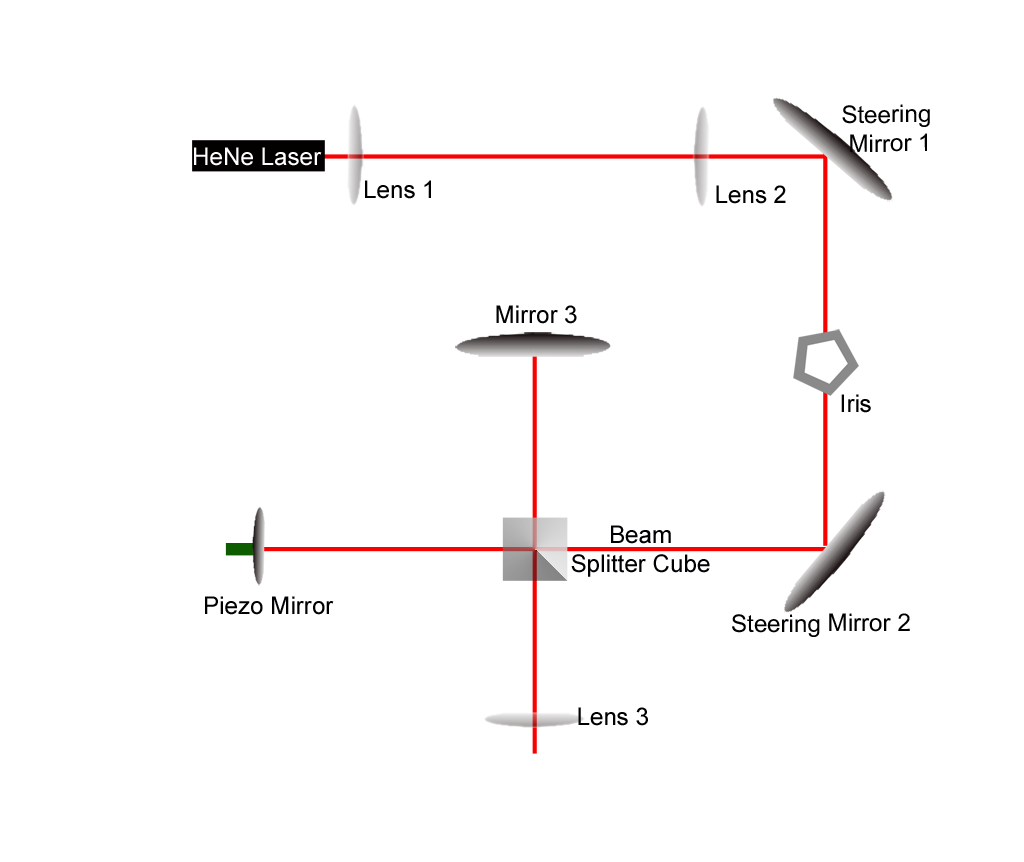
\includegraphics[width= 3.25 in]{interferometer}
\caption{Basic Diagram of our Michelson Interferometer}
\label{fig:interferometerdiagram}
\end{figure}


	With a Michelson interferometer you can measure distances and refractive indices of test materials introduced into the beam path. To make the measurements remember that light is an electromagnetic wave that can be described by the scalar equation
	\begin{align}\label{eqn:EMWave}
		\nonumber E(x,y,z,t) &= a\cos{2\pi(\nu t-\frac{z}{\lambda})} \\
		&= a\cos{\omega t-kz}
	\end{align}
with $\omega=2\pi\nu$ being the angular frequency and $\nu$ the wave frequency, $\emph{k}=\frac{2\pi}{\lambda}$ is the propagation constant and $\lambda$ is the wavelength in space.  

	By switching to exponential it is easier to work with the wave equation. Based on Euler’s formula we have that 
	\begin{equation}\label{eqn:Euler's}
		e^{i\theta} = \cos{\theta} + i \sin{\theta}
	\end{equation}
and since $\cos(\theta)=\Re\{e^{i\theta}\}$ we can rewerite our wave formula in the following form
	\begin{align}\label{eqn:TrigEMWave}
		\nonumber E(x,y,z,t) &=\Re\{a e^{-ikz} e^{i\omega t}\} \\
		\nonumber &=\Re\{a e^{-i\phi} e^{i\omega t}\} \\
		&=\Re\{A e^{i\omega t}\}
	\end{align}
where the phase $\phi=kz$ and the amplitude of the wave $A=ae^{-i\phi}$. The total amplitude of 2 interfering waves at a point is the sum of the amplitude of each individual wave.
	\begin{equation}\label{eqn:Amplitude}
		A_{T}=A_{1}+A_{2}
	\end{equation}
Based on whether it is constructive or destructive interference $A_T$ can be the sum or the difference of the amplitudes. 

	The intensity of the wave is proportional to the total amplitude squared, 
	\begin{align}\label{eqn:Intensity}
	\nonumber I_{T} &=|A_{T}|^{2} \\
	\nonumber &=(A_{1}+A_{2})(A_1^*+A_2^*) \\
	\nonumber &=|A_1|^{2} +|A_2|^{2} +A_1 A_2^* +A_2 A_1^* \\
		I_{T} &=I_1 + I_2 +2(I_1 I_2)^{1/2} \cos{\Delta \phi}
	\end{align}

	For the Michelson Interferometer in this lab you are starting from one source, therefore the initial amplitudes and wavelengths are the same. The only phase difference, between the two beams, affecting the amplitude comes from a difference in the beam paths. 
	\begin{align}\label{eqn:offset}
		\nonumber \Delta \phi &=\frac{2\pi}{\lambda} \Delta p \\
		\nonumber \Delta p &=\sum(n_2 d_2)-\sum(n_1 d_1) \\
				&=n_2 d_2 - n_1 d_1
	\end{align} 
In the above equation $n$ is the refractive index of the medium, $d$ is the lenght of the beam path. Since the medium through which the beam paths are traveling is the same, air, then the index of refraction $n_1$ is equal to $n_2$ making the beam paths offset 
	\begin{align}\label{eqn:offset2}
		\nonumber \Delta p &=n(d_2 - d_1) \\
		\Delta \phi &=\frac{2\pi n}{\lambda}(d_2 -d_1) \text{\textbf{.}}
	\end{align}

	Substituting the beam offset into equation 5 the intensity becomes:
	\begin{align}\label{Intensity2}
		\nonumber I_{T} &=I_1 +I_2 +2(I_1 I_2)^{1/2} \cos{\frac{2\pi n}{\lambda}(d_2 -d_1)} \\
		\nonumber &=2I +2I\cos{\frac{2\pi n}{\lambda}(d_2 -d_1)} \\
		\nonumber &=2I(1+\cos{\frac{2\pi n}{\lambda}(d_2 -d_1)})
	\end{align}
